\documentclass[letterpaper,10pt]{article}

%\setlength{\parindent}{0in}
%\usepackage{fullpage} 
\usepackage{amsmath}
\usepackage{amssymb}
\usepackage{enumerate}
\usepackage{graphicx}
\usepackage[table]{xcolor}
\usepackage{dcolumn}
\oddsidemargin 0.0in
\textwidth 6.5in
\newcolumntype{.}{D{.}{.}{-1}}
\newcommand*{\myalign}[2]{\multicolumn{1}{#1}{#2}}

%opening
\title{Homework}
\author{Steve Mazza}
%\date{July 22, 2013}

\begin{document}
\maketitle

\section*{Final Project}
\subsection*{Problem 2}
The computed deficiency angle is $90^{\circ}$. 
\subsubsection*{Solution 1}
 One solution is to choose a pole-zero pair that cancels a pole at the origin: $G_{c}(s) = \dfrac{s+0}{s+2}\times\dfrac{1}{s^{2}}$.
This corrects the angle deficiency as follows: $135 + 135 + 45 - 135 = 180$.

\subsubsection*{Solution 2}
Another solution is $G_{c}(s) = \dfrac{s+0.5}{s+3}\times\dfrac{1}{s^{2}}$.
This corrects the angle deficiency as follows: $135+135+30-120=180$.

\subsubsection*{Root-Loci Plot}
\begin{center}
	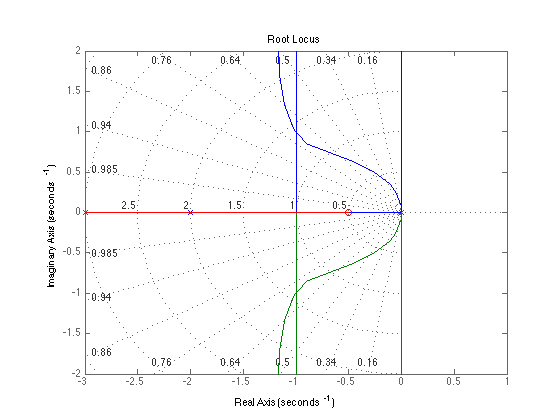
\includegraphics[scale=0.75]{2-rlocus.png}
\end{center}
Both solutions pass through $s=-1\pm j$ with a gain of $K=4$.

\subsubsection*{System Responses}

\begin{center}
	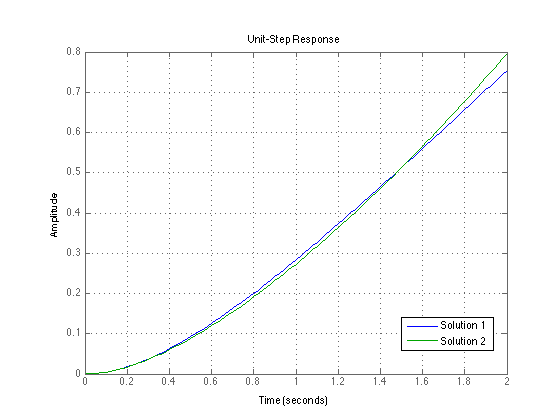
\includegraphics[scale=0.65]{2-unit-step.png} \\
	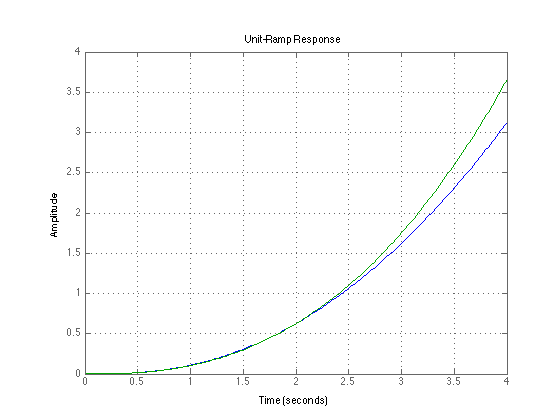
\includegraphics[scale=0.65]{2-unit-ramp.png} \\
	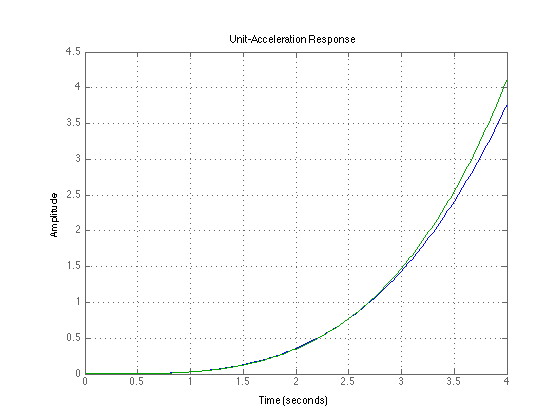
\includegraphics[scale=0.65]{2-unit-accel.png}
\end{center}

Given the response curves, solution 1 (pole-zero cancellation) seems the better option.

\subsection*{Problem 3}
We calculate the steady state error, $E_{ss}$\dots
\[E_{ss} = \dfrac{10\times 20}{10\times 20+820}\approx 0.2\]
This gives us a desired steady state error of $E_{ss_{c}} = 0.02$.  Then we use $E_{ss_{c}}$ to calculate the desired pole-zero ratio\dots
\[\dfrac{z}{p} = \dfrac{10\times 20 - 0.02\times 10\times 20}{0.02\times 820}\approx 11.95\]
We use a rule of thumb to find the placement of our zero, $z = 20/50 = 0.4$ and apply our pole-zero ratio to arrive at
\[\dfrac{z}{p} = \dfrac{0.4}{0.03}\]
To get closer to the origin, we ignore manufacturing constraints and also choose
\[\dfrac{z}{p} = \dfrac{0.04}{0.003}\]

\subsubsection*{Root-Locus Plot}
\begin{center}
	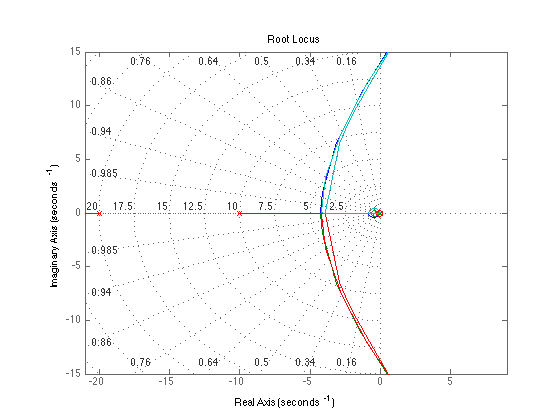
\includegraphics[scale=0.75]{3-rlocus.png}
\end{center}

\subsubsection*{System Responses}
\begin{center}
	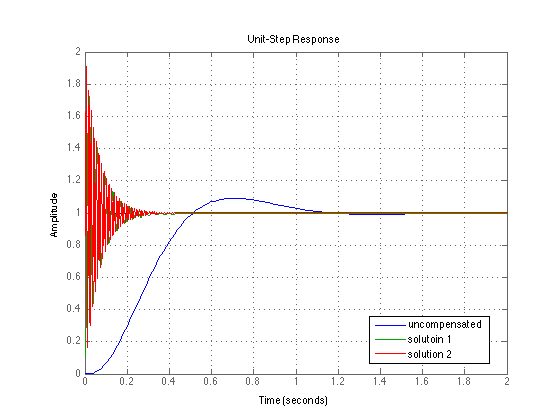
\includegraphics[scale=0.6]{3-unit-step.png} \\
	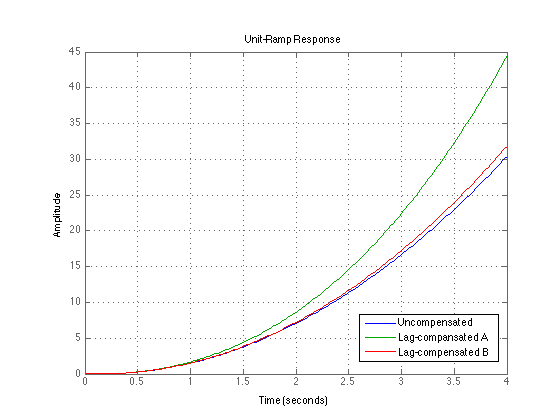
\includegraphics[scale=0.6]{3-unit-ramp.png}
\end{center}

\end{document}